%%%%%%%%%%%%%%%%%%%%%%%%%%%%%%%%%%%%%%%%%
% University Assignment Title Page 
% LaTeX Template
% Version 1.0 (27/12/12)
%
% This template has been downloaded from:
% http://www.LaTeXTemplates.com
%
% Original author:
% WikiBooks (http://en.wikibooks.org/wiki/LaTeX/Title_Creation)
%
% License:
% CC BY-NC-SA 3.0 (http://creativecommons.org/licenses/by-nc-sa/3.0/)
% 
% Instructions for using this template:
% This title page is capable of being compiled as is. This is not useful for 
% including it in another document. To do this, you have two options: 
%
% 1) Copy/paste everything between \begin{document} and \end{document} 
% starting at \begin{titlepage} and paste this into another LaTeX file where you 
% want your title page.
% OR
% 2) Remove everything outside the \begin{titlepage} and \end{titlepage} and 
% move this file to the same directory as the LaTeX file you wish to add it to. 
% Then add \input{./title_page_1.tex} to your LaTeX file where you want your
% title page.
%
%%%%%%%%%%%%%%%%%%%%%%%%%%%%%%%%%%%%%%%%%
%\title{SemesterProject}
%----------------------------------------------------------------------------------------
%	PACKAGES AND OTHER DOCUMENT CONFIGURATIONS
%----------------------------------------------------------------------------------------

\documentclass[12pt]{article}
\usepackage[english]{babel}
\usepackage[utf8x]{inputenc}
\usepackage{amsmath}
\usepackage[version=4]{mhchem}
\usepackage{blindtext}
\usepackage{chemfig}
\usepackage{graphicx}
\usepackage{float}
\usepackage{multicol}
\usepackage[colorinlistoftodos]{todonotes}
\usepackage{setspace}
\renewcommand{\contentsname}{Come one!}
\renewcommand{\contentsname}{Table of Content}

\begin{document}

\begin{titlepage}

\newcommand{\HRule}{\rule{\linewidth}{0.5mm}} % Defines a new command for the horizontal lines, change thickness here

\center % Center everything on the page
 
%-------------------------------------------------------------- --------------------------
%	HEADING SECTIONS
%----------------------------------------------------------------------------------------
{\setstretch{1.5}\textsc{\LARGE Swiss Federal Institute of Technology Zürich  }\\[1cm]
}

\textsc{\Large Semester Project}\\[0.5cm] % Major heading such as course name
\textsc{\large Alex goes LBB}\\[0.5cm] % Minor heading such as course title

%----------------------------------------------------------------------------------------
%	TITLE SECTION
%----------------------------------------------------------------------------------------

\HRule \\[0.4cm]
{\setstretch{3}  {\huge \bfseries Biocompatible and conductive fiber for implant applications}}\\[0.4cm] % Title of your document

\HRule \\[1.5cm]
 
%----------------------------------------------------------------------------------------
%	AUTHOR SECTION
%----------------------------------------------------------------------------------------

\begin{minipage}{0.4\textwidth}
\begin{flushleft} \large
\emph{Author:}\\
Alexandre \textsc{Meier}\\
\textcolor{white}{Yeah}\\
\textcolor{white}{Yeah}
\end{flushleft}
\end{minipage}
~
\begin{minipage}{0.5\textwidth}
\begin{flushright} \large
\emph{Supervisors:} \\
Aline \textsc{Renz}\\
Dr. Jaehong \textsc{Lee}\\[0.1cm]
Prof. Dr. Janos \textsc{Vörös}
\end{flushright}
\end{minipage}\\[2cm]


%----------------------------------------------------------------------------------------
%	DATE SECTION
%----------------------------------------------------------------------------------------

{\large November, 2018}\\[2cm] % Date, change the \today to a set date if you want to be precise

%----------------------------------------------------------------------------------------
%	LOGO SECTION
%----------------------------------------------------------------------------------------
\centerline{
\includegraphics[scale=0.9]{ETH_LBB.PNG}}


% \includegraphics{}\\[1cm] % Include a department/university logo - this will require the graphicx package
 
%----------------------------------------------------------------------------------------

\vfill % Fill the rest of the page with whitespace

\end{titlepage}


\begin{abstract}
TODO: Enter Abstract.
\end{abstract}

\newpage

\tableofcontents

\newpage

\section{Introduction}

TODO: Introduction 

\section{Theory}

\subsection{Polyurethane}

Polyurethanes (PUR) are biocompatible and biostable polymers, with urethane as the characteristic group. Due to most PUR being classically synthesized using polycondensation of diisocyanates with alcohols and amines, two side groups are introduced. This leaves the option for functionalization, depending on the requirement of the application. 

On one hand, they're moldable and have favourable tensile and fatigue properties, all of which makes them a suitable choice of material for the development of most complex biomedical devices. Until now, PUR has been extensively studied in the context of small vascular shunts and cardiac assist devices, where the thromboresistant property of the PUR fit formidable. Under most physiologic conditions, PUR are degradation resistant and can handle stresses very well. [Ulery] 
On the other hand, PUR's main usages are far more mundane. Due to being adhesive it is mainly used as grounding for painting. During everyday life, one may encounter PUR as usual kitchen sponges, filling in car seats and spandex.

However, PUR, is not electrically conductive. This makes it impossible to introduce electrical functionalities with pure PUR implants, like in-device monitoring, wireless implant-environment-communication or conductivity-coupled strain sensing.


\subsection{Gold Salt}

When having to decide, which conductive material to use, noble metals seem to host quite some promising candidates. The two main properties we wanted to base our decision on are biocompatibility and conductivity. Silver is highly conductive, but also severly cytotoxic. Platinum, on the other hand, is not conductive, but biocompatible, even though there's a growing body of evidence that proves otherwise. As a consequence we decided on using gold, as it provides the best compromise between conductivity and biocompatibility. Also there is robust evidence, that gold stays biocompatible, even as gold nanoparticles (AuNP). This is especially important, when considering that this is the relevant size range for this work. [Liu][Shukla]

Due to fiscal reasons, we had an interest in increasing the efficiency. This is typically done by minimizing the amount of substance that is wasted in non-targeted interactions. Gold in bulk is highly inert and therefore difficult to incorporate in a defined chemical approach, whereas the ionic form is a well studied agent in RedOx-reactions (i.e.the method that was chosen in this work).  The increase in efficiency can be achieved using a spatially selective approach with gold salt, where only the fiber is decorated with gold.

Gold(III) chloride trihydrate was therefore the reagent of choice.

\subsection{Reduction agent}


The reaction we wanted to happen, is the reduction of gold. Gold in bulk electrically conductive and promises better properties for usage.

Redox-Reaction (Two main ingredients, reduction and oxidation agent)

Draw redox-equation

The criteria for our reduction agent. Not to aggressive, because we want to limit reaction to gold. Polyurethane cannot be modified. should be able to reduce gold. 
cheap and easily accessible

optimally biocompatible



\section{Methods}
\label{sec:Methods}

\subsection{Manufacturing}

\subsubsection{Preparation of reagent}

All reagents were of analytic grade and were used as received from the suppliers without further  purification. Every chemical was bought from Sigma Aldrich, unless stated otherwise. 
Next for facilitation we introduced the formula making use of stoichiometry:

    $$\frac{m'\cdot v\cdot M}{1000} = m(m',v,M), $$

where ~$m'$ denotes the molecular weight of the reagent, ~$v$ the desired end-volume of the solution, ~$M$ the molar concentration and ~$m$ the needed amount of the substance with unit 'grams', assuming the chemical to be pure. (Example: We want to make 4ml (~$= v$) of solution with \ce{NaOAc} (~$m'_{\ce{NaOAc}}= 82.03 \frac{g}{mol}$) at a concentration of 0.25 M (~$= M$). We now know, that we need to dilute $m \approx 82mg$ \ce{NaOAc} in 4ml of solvent!) 

\newpage 


\paragraph{Gold solution}

We used Gold(III) chloride trihydrate, dissolved in ethanol (EtOH). The concentration, unless stated otherwise, was 0.25M and was prepared using the formula given above.


\paragraph{Reduction agent solution}

TODO: Enter Reduction Agent Table

From the identified reduction agents, the reagent was produced by diluting it in H20dd until the concentration given was reached. Were the reduction agent was light-sensitive, we put aluminium-foil around the containing reservoir.

\subsubsection{Sample Fabrication}

Define Experiment. We identified 5 independent variables that can be changed.


\begin{multicols}{2}
\begin{itemize}
    \item Gold concentration (\textit{c\textsubscript{gold}})
    \item Gold immersion time (\textit{t\textsubscript{gold}})
    \item Choice of reduction agent
    \item Reduction agent concentration (\textit{c\textsubscript{Red}})
    \item Reduction agent immersion time (\textit{t\textsubscript{Red}})
\end{itemize}
\end{multicols}




\paragraph{Initial Protocol}

\begin{enumerate}
    \item Define which parameters are fixed and which are experimental parameters. Define range you want to investigate.
    
    \item Define concise naming concept, which allows every sample to be uniquely identified.
    
    \item Per sample reserve two petri dishes (PD) and label them in accordance with above mentioned concept. You might add the tag "Pre" and "Post" to existing description. (\textit{PDPre/PDPost}).
    
    \item Put 0.75ml of Gold Solution with \textit{c\textsubscript{gold}} in small, optimally non-translucent viol to account for the light-sensitivity of the gold salt (\textit{Viol}). One viol per sample you wish to investigate. Further decrease of translucency can be achieved by putting aluminium around viol.
    
    \item Put fiber in corresponding \textit{viol} and let immerse according to your defined \textit{t\textsubscript{gold}}.
    \item Take fiber out \textit{viol} and put in \textit{PDPre} to let dry. Note change in colour and/or structure. Experience shows that 30 minutes is sufficient.
    
    \item Gently pour 1ml of reduction agent solution with \textit{c\textsubscript{Red}} over fiber, while making sure the whole fiber is immersed. Note colour gradient in fiber and temporal resolution. Let immerse according to defined \textit{t\textsubscript{Red}}.
    
    \item After passing of time, transfer the fiber gently to \textit{PDPost}, where it will dry.
    \end{enumerate}
    
    \begin{center}
        This marks the end of the fiber fabrication.
    \end{center}


\paragraph{Optimized Protocol} \hfill\newline

1. / 2. are identical to initial protocol.

\begin{enumerate}
\setcounter{enumi}{2}
    
    \item Per sample reserve one petri dish (PD) and one glass slide (GS). Label them in accordance with above mentioned concept, whereas you might add the tag "Pre" to the PD and "Post" to GS description. (\textit{PDPre/GSPost}).
    
    \item Put 0.75ml of Gold Solution with \textit{c\textsubscript{gold}} in small, optimally non-translucent viol to account for the light-sensitivity of the gold salt (\textit{Viol}). One viol per sample you wish to investigate. Further decrease of translucency can be achieved by putting aluminum around viol.
    
    \item Put fiber in corresponding \textit{viol} and let immerse according to your defined \textit{t\textsubscript{gold}}.
    \item Take fiber out viol and put in \textit{PDPre} to let dry. Note change in color and/or structure. Experience shows that 30 minutes is sufficient.
    
    \item Gently pour 1ml of reduction agent solution over fiber, while making sure the whole fiber is immersed. Note color gradient in fiber and temporal resolution. Let immerse according to defined \textit{t\textsubscript{Red}}.
    
    \item After passing of time, transfer the fiber gently to \textit{GSPost}, where it will dry.
    \end{enumerate}
    
    \begin{center}
        This marks the end of the fiber fabrication.
    \end{center}

\subsection{Measurement}

\subsubsection{Preparation}
Prerequisites:
\begin{multicols}{2}
\begin{itemize}
    \item Sample with size $l$
    \item A small piece of paper
    \item 8 Pieces of Tape
    \item Silver Epoxy
    \item Derubberized Cable
\end{itemize}
\end{multicols}

Protocol:

\begin{enumerate}
    \item On piece of paper, put 1 piece of tape (Tape 1) on each side with distance $d < l$ from each other
    \item Now fix both ends of the sample gently without stretching (!) on Tape 1 with another piece of tape (Tape 2).
    \item Then, put free end of cable on end of sample, which is free and over Tape 1. Establish contact and fix cable with Tape 3.
    \item Put Silver Epoxy on sample-cable-interface to facilitate sample-cable-transmission. Bake at 80\textdegree C for 2h. After taking out the oven, put tape 4 perfectly aligned with the medial edge of Tape 1.
\end{enumerate}

    \begin{center}
    TODO
    Refer to actual figure (Add label, fix picture organisation.)
    TODO
    
See figure number \ref{fig:MeasPrep} in Appendix for visual description of resistance measurement preparation.
    \end{center}


\subsubsection{Resistance Measurements}
TODO describe Iterative Strain Protocol, including general assumptions and execution of protocol \myworries{TODO}
\section{Results \& Discussion}
\label{sec:ResAndDisc}


\subsection{Identification of reduction agent}

\myworries{Put up list of reduction agents tried}
\myworries{Add label!!}

NaBH4 has been described in the literature to produce gold nanoparticles in tunable sizes, depending on the ratio between NaBH4- and gold concentration \cite{NaBH4UsedForGoldNP}. To account for the already acidic environment coming from the gold salt itself, we introduced another group, that consisted of a combination of \ce{NaBH4} and \ce{NaOH} by 1:1 ratio, where NaOH as a sodium base, should moderate the reduction to happen in a less acidic environment.
Hydroxylamine as reducing agent is widely known and has already been described in the context of production of silver colloids \cite{Leopold}.  
As proposed by work done by Goia, Kimming and Turkevich, we added Ascorbic Acid (AscAc), Citric Acid (CitrAc) and a reducing sugar (here: Glucose) to the tested reduction agents. \cite{Goia, Kimling, Frens}

There were 3 samples per reduction agent. Following the heuristic approach, where we optimised the knowledge gain per sample-ratio, we subdivided each group by three different reduction agent immersion times, which were 20 minutes, 40 minutes and 2 hours, respectively. This means that every permutation-group [Reduction Agent/Reduction agent Immersion Time] had one sample.

\myworries{AddGraph of $t_{Red}$ v $R_0$}\\
\myworries{Add Label too}

\paragraph{NaBH4}
During Production we followed the standard procedure with the concentration stated. \ce{NaBH4} is known to hydrolyse in solute and therefore, the intended reactivity is reduced. To decrease premature hydrolation, the \ce{NaBH4}-solution was prepared just before usage and put on ice between production and use. Upon immersion of fiber in \ce{NaBH4}, the production of bubbles could be observed as can be seen in figure \ref{unknown-marker} \myworries{Add Label for Bubbly picture in Appendix.}.

The following equation describes the oxidation-half reaction in this sample:

\begin{center}
\schemestart 
\ce{[BH4]-} + \ce{H+} + 3\ce{H2O}   \arrow{->} \ce{H3BO3} + 4\ce{H2{(g)}}, 
\schemestop\par 
\end{center}

With the stated concentration in table \ref{unknown-marker}, we were able to measure conductivity in all three samples as can be seen in figure \ref{unknown-marker}. We acknowledge the fact that one sample is not sufficient for any significant statement. Nevertheless, we see a tendency of a decreasing resistance when increasing the immersion time, exhibiting a time-dependency in this relation. As a general rule, chemical reactions are known to target a certain ratio between reactant and product \myworries{add reference}. This principle could explain the time-dependency. The produced hydrogen gas evades the liquid reaction solution continuously as seen in picture \myworries{addRef for bubbly Picture}. This imbalance between reactant and product is counter-steered by a shift towards the product side present in the solution, which over time would lead to a steady-state, where the increased concentration of \ce{H3BO3} compensates for the lack of \ce{H2{(g)}}. However, as long the reaction did not reach the steady state, gold atoms will be produced and nuclei will grow. Implicitly this includes the decrease in resistance whose end is marked by a critical point that is governed by reaching the ratio described above or the nanoparticle size.

Scanning Electron Microscopy (SEM) pictures showed a largely heterogeneous distribution of nanoparticles. However, EDS analysis of the crosssection of the fiber reveals gold coating. \myworries{Add Ref}

\paragraph{\ce{NaBH4}/\ce{NaOH}}
\myworries{Check if there are lab-pictures. Refer to them. We did not take SEM/EDS pictures}.


\paragraph{Hydroxylamine}
Production was done according to protocol and with the concentration stated. No conductivity was measured. Nevertheless, SEM pictures revealed successful reduction of gold into round nanoparticles that at some location formed large colloids. \myworries{Add Ref for HyA Picture} Following the principle of Occam's razor, we hypothesise that in the process of the reaction, eventually, the nanoparticles grew to big and subsequently "fell off" the fiber. This explains the phenomenon of no conductivity without any particles.


\paragraph{Ascorbic Acid}
Production was done according to protocol and with the concentration stated. The conductivity measured was 25-43 $\Omega$ and outperforms the next best reduction agent by almost 4 orders of magnitude in the described setup. 


\paragraph{Citric Acid}
The citric acid protocol was slightly changed, upon suggestion by work done by Kimling \cite{Kimling} to include an initiating element to facilitate the formation of nuclei, which then - according to explanation found in chapter \ref{subsec:Perc} - should suffice for produced gold atoms to associate to the nucleus and finally nanoparticles to grow. The identified initiators where heat-exposition and UV-irradiation. For each of those two subgroups, only one sample was prepared.

We prepared the heat exposition group following standard procedure up until the immersion of the fiber in the reduction agent (i.e. citric acid in this case). Using the hot plate, we prepared the citric acid solution to be between 100-120 \degree C, before the fiber was immersed. Over the course of 35 minutes the solution changed from faintly blue and turbid to a clear solution with red particles floating in the solution. A picture of the solution after letting it cool down is shown on page \ref{unknown-marker} \myworries{Add Citric Acid Picture}. The described behaviour replicates the description by Frens\cite{Frens}. Yet, we were not able to measure current.

Using a Demetron Optilux 500, we irradiated one sample after immersion  citric acid solution. The picture on page \ref{unknown-marker} \myworries{Add Picture of Bubbly and reference it} shows the emergence of bubbles at the fiber-solution-interface during irradiation. Comparison with a control citric acid group, where bubble formation was absent, leads to conclusion the phenomenon is caused by the irradiation. However, the integrity of the fiber was impaired. Attempts to take it out the petri dish, showed that the polyurethan fiber was thinned out substantially and sticked on the petri dish. Obviously, there was an influence of the UV-light on the fiber. Further experiments with variable irradiation times and/or intensities, could lead to a more thorough explanation. No conductivity measurement was done in this group.


\myworries{Add UV-Fiber Picture}


\paragraph{Glucose}
Upon suggestion by Kimling \cite{Kimling}, we kept the reduction agent solution at around 30 \degree C during the whole immersion time, using the hot plate. After 15 minutes, some of the solution clearly visible condensed on the closing lid of the petri dish \myworries{Add Picture of PetriDish}. We were not able to measure any conductivity in this sample. However, SEM pictures revealed the formation of gold nanoparticles. Upon further magnification, the peculiar structure of those nanoparticles became visible. The nanoparticles had cracks, which in bigger ones would reveal the pitch black cavities. Due to technical difficulties, the SEM in this setup is not able to image those, but it looks like the nanoparticles are hollow, with the apparent nanoparticles being merely a nanoparticle-shell. The cracks can also be seen on the surface of the fiber. Further experiments with variable temperature and heating times maybe can provide more information on the origin of this behaviour.\\

%\hfill \newline

All reduction agents tested effectuated a change in fiber colour when following the described protocol. As indicated in chapter \ref{subsec:GoldSalt}, this shows that in the experimental setup the reduction of gold was successful. If not stated otherwise the sample did not lead to any behaviour that was worth noting, neither when analysing the reduction agent solution after sample immersion or the fiber by eye.

However, due to the fact no reduction agent but \ce{NaBH4} and \ce{AscAc} did lead to conduction in our fibers, we also conclude that the sheer reduction of gold is not enough to functionalise our fiber with conductivity. In order to explain the relation ship between the reduction agents and the conductivity of the fiber, we have to introduce another metric, which we propose to be the quality of the gold nanoparticles.

\myworries{Here SEM/EDS Pictures Pictures}

As can be seen in the SEM pictures \myworries{ref The SEM pictures} we can partially explain the conductivity by uniformity in spatial distribution and size of the nanoparticles. Further experiments could elucidate which of these factors weigh how much into the equation that explains conductivity in our fibers. 

\subsection{Optimisation}
Encouraged by the good results we decided to optimise for AscAc before making baseline resistance tests for new reduction agents. Additionally, we now took not only the baseline resistance into account but also its behaviour when put under strain stress. This measurement reflects now more the true use case and should reduce misdirected optimisation. The five independent variables defined in chapter \ref{subsec:SampleFab} are now reduced to four. If not different stated, following applies: \begin{center}$c_{AscAc}=0.19M$, $t_{AscAc}=20min$, $c_{Gold}=0.25M$ and $t_{Gold}=1h$
\end{center}
Next we assigned each of those independent variables an anticipated effect size. By intuition we assigned them in the following order, where $>$ marks "has the bigger anticipated effect size than":

\begin{equation}
    c_{AscAc} > c_{Gold} > t_{AscAc} > t_{Gold}
\end{equation}

\subsubsection{Variation of Gold Concentration}

Gold concentration was varied to be $0.025M, 0.25M$  and $0.6M$, respectively.

\begin{figure}[H]
    \centerline{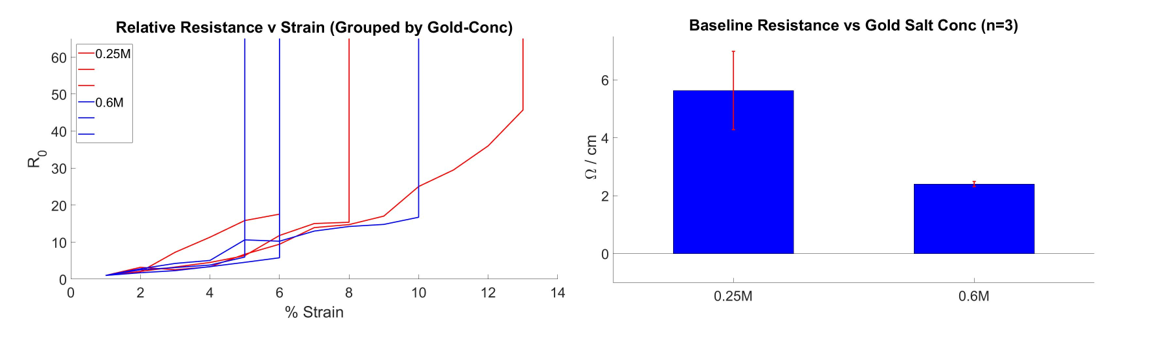
\includegraphics[scale=0.7]{./pic/R0vGoldConc.PNG}}
    \caption{Variation of Gold Concentration}
    \label{fig:GoldConc}
\end{figure}

The $0.025M$-samples did not lead to measurable conduction. The result of the baseline resistance seemingly favours a higher gold concentration. However, the data of strain resistance does not allow for a similarly clear statement, neither when plotting the absolute resistance nor when plotting the normalised one, as we see in figure \ref{fig:GoldConc}, left. The sudden peak out of the plotted range mark the critical point, where conductivity in the fiber was lost and no current was measured. Relaxation of strain also led to regain of measurable conductivity similar to a priori values (not shown).

\subsubsection{Variation of Reduction Agent}


\hfill \newpage
\section{Outlook}
\label{sec:Outlook}

Our outlook on the described technology is positive. Using Ascorbic acid, the water-soluble Vitamin C, as a reducing agent, we have been successful in producing fibres that show linear strain-resistance behaviour in a physiological range of 20\%. Yet, there is a high variability in exhibited strain-resistance behaviour, which might hinder the direct integration in a more complex device. However, upon identification of the governing factors, we can minimise variability and increase reproducibility of previously mentioned behaviour.\\
The suggestions in advancement are two-fold and can be divided into either further optimization of the already described protocol parameters or by modification of the fiber production protocol.\\
When optimising the existing protocol, it becomes apparent that further inspection is needed. In order to gain insight and describe better the dynamic of the conducting gold particles during stretching, we suggest to image the fibres upon strain by SEM. Then with new information, we can suggest further advancements accordingly. One possible outcome could be that upon stretching the previously homogeneously distributed gold nanoparticles divide into a few big compartments which are interspaced by non-conducting areas, ultimately failing conduction. Since this could be a sign of missing or heterogenous adhesion on the fibre surface, we could propose to modify fibre  surface roughness. Furthermore, we also see potential in furhter standardizing both resistance measurement protocols (Preparation/Measurement).\\
When modifying the fibre production, we could propose to enclose the fiber in an elastomeric layer to allow for increased stability and sustained integrity of the conducting network. Another suggestion could be to introduce an in-situ reduction process similar to work done by Wei, where by fully immersing the non-conducting polymer in the reaction space, Wei's group was able to increase conductivity by 3-5 fold, when comparing it to conventional approaches.\cite{Wei}







\section{Some \LaTeX{} Examples}
\label{sec:examples}
\subsection{Sections}

Use section and subsection commands to organize your document. \LaTeX{} handles all the formatting and numbering automatically. Use ref and label commands for cross-references.



\subsection{Comments}

Comments can be added to the margins of the document using the \todo{Here's a comment in the margin!} todo command, as shown in the example on the right. You can also add inline comments too:

\todo[inline, color=green!40]{This is an inline comment.}

\subsection{Tables and Figures}

Use the table and tabular commands for basic tables --- see Table~\ref{tab:widgets}, for example. You can upload a figure (JPEG, PNG or PDF) using the files menu. To include it in your document, use the includegraphics command as in the code for Figure~\ref{fig:frog} below.

% Commands to include a figure:
\begin{figure}[h!]
\centering
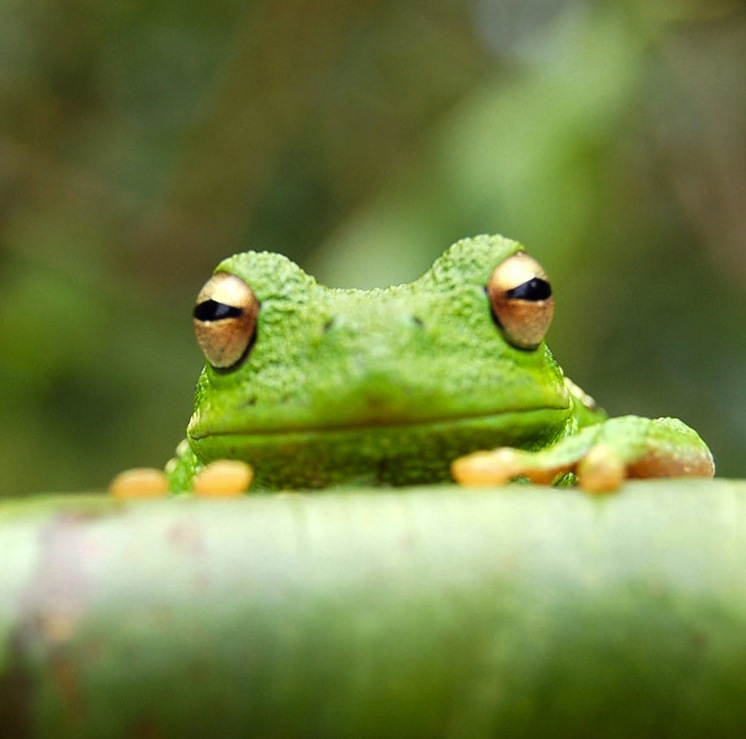
\includegraphics[width=0.5\textwidth]{frog.jpg}
\caption{\label{fig:frog}This is a figure caption.}
\end{figure}

\begin{table}[h!]
\centering
\begin{tabular}{l|r}
Item & Quantity \\\hline
Widgets & 42 \\
Gadgets & 13
\end{tabular}
\caption{\label{tab:widgets}An example table.}
\end{table}

\subsection{Mathematics}

\LaTeX{} is great at typesetting mathematics. Let $X_1, X_2, \ldots, X_n$ be a sequence of independent and identically distributed random variables with $\text{E}[X_i] = \mu$ and $\text{Var}[X_i] = \sigma^2 < \infty$, and let
$$S_n = \frac{X_1 + X_2 + \cdots + X_n}{n}
      = \frac{1}{n}\sum_{i}^{n} X_i$$
denote their mean. Then as $n$ approaches infinity, the random variables $\sqrt{n}(S_n - \mu)$ converge in distribution to a normal $\mathcal{N}(0, \sigma^2)$.

\subsection{Lists}

You can make lists with automatic numbering \dots

\begin{enumerate}
\item Like this,
\item and like this.
\end{enumerate}
\dots or bullet points \dots
\begin{itemize}
\item Like this,
\item and like this.
\end{itemize}

We hope you find write\LaTeX\ useful, and please let us know if you have any feedback 
using the help menu above.
\clearpage
\phantomsection
\appendix
\section{\\Figures}


\begin{figure}[hb]
\centerline{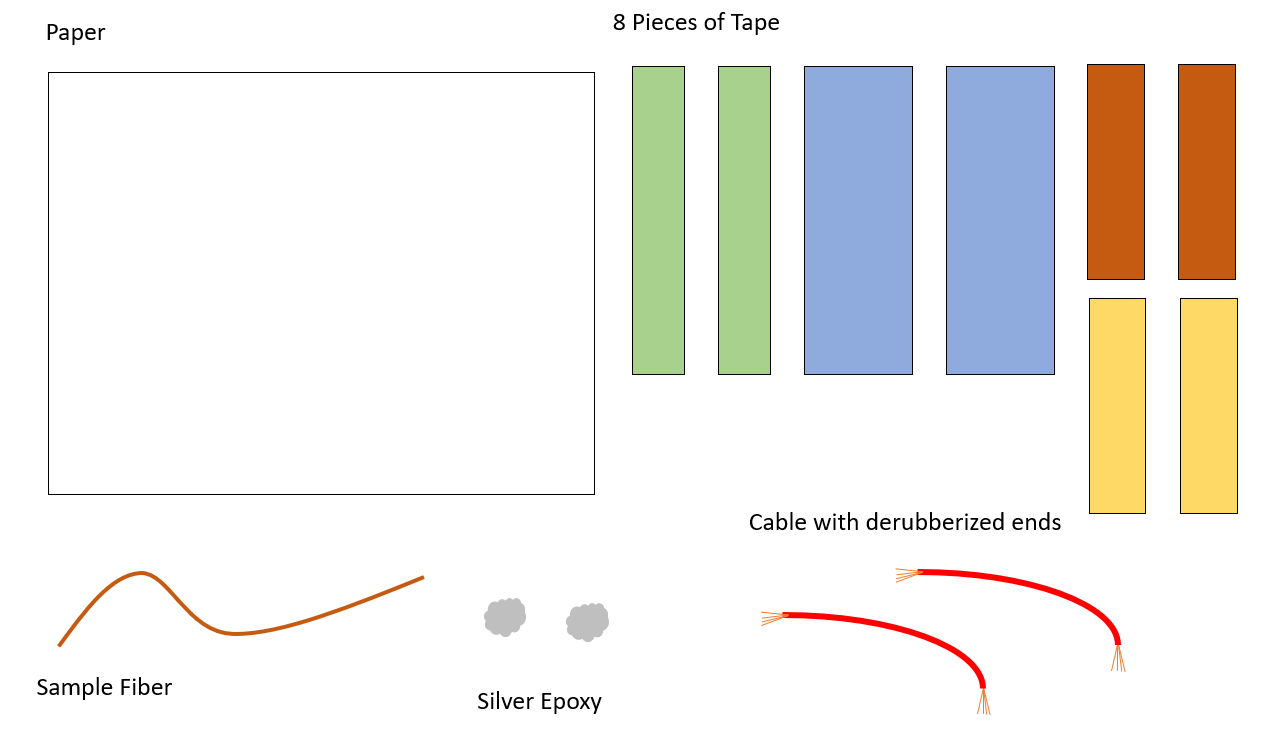
\includegraphics[scale=0.2]{Meas_Prep_1.PNG}}
\caption{\label{fig:MeasPrep1}That shit cray.}
\end{figure}

\begin{figure}[hb]
\centerline{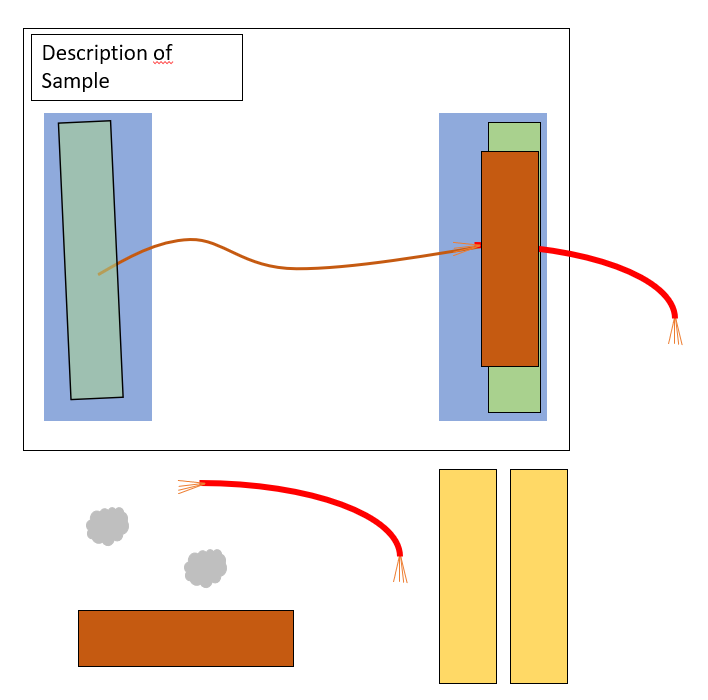
\includegraphics[scale=0.2]{Meas_Prep_2.PNG}}
\caption{\label{fig:MeasPrep2}That shit cray.}
\end{figure}

\begin{figure}[hb]
\centerline{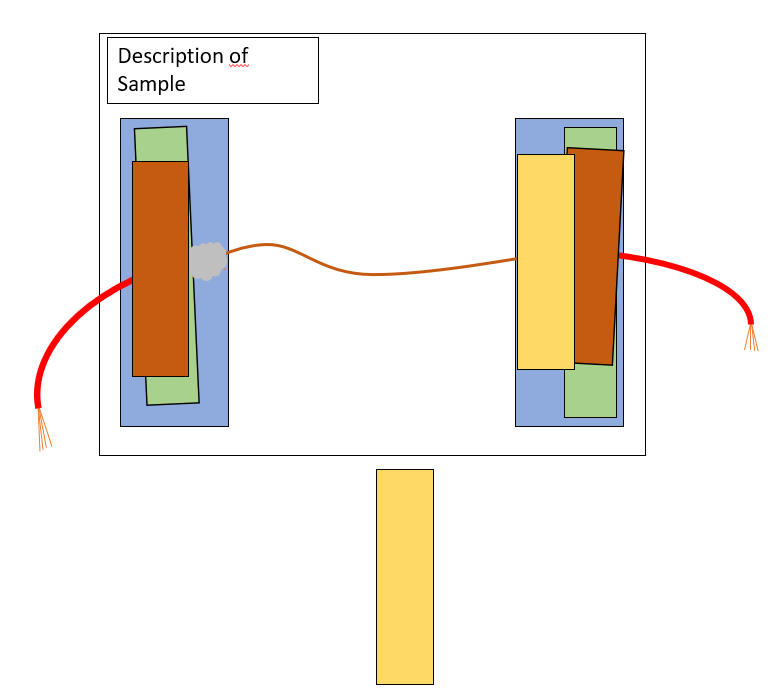
\includegraphics[scale=0.2]{Meas_Prep_3.PNG}}
\caption{\label{fig:MeasPrep3}That shit cray.}
\end{figure}


\begin{figure}[hb]
    \centering
    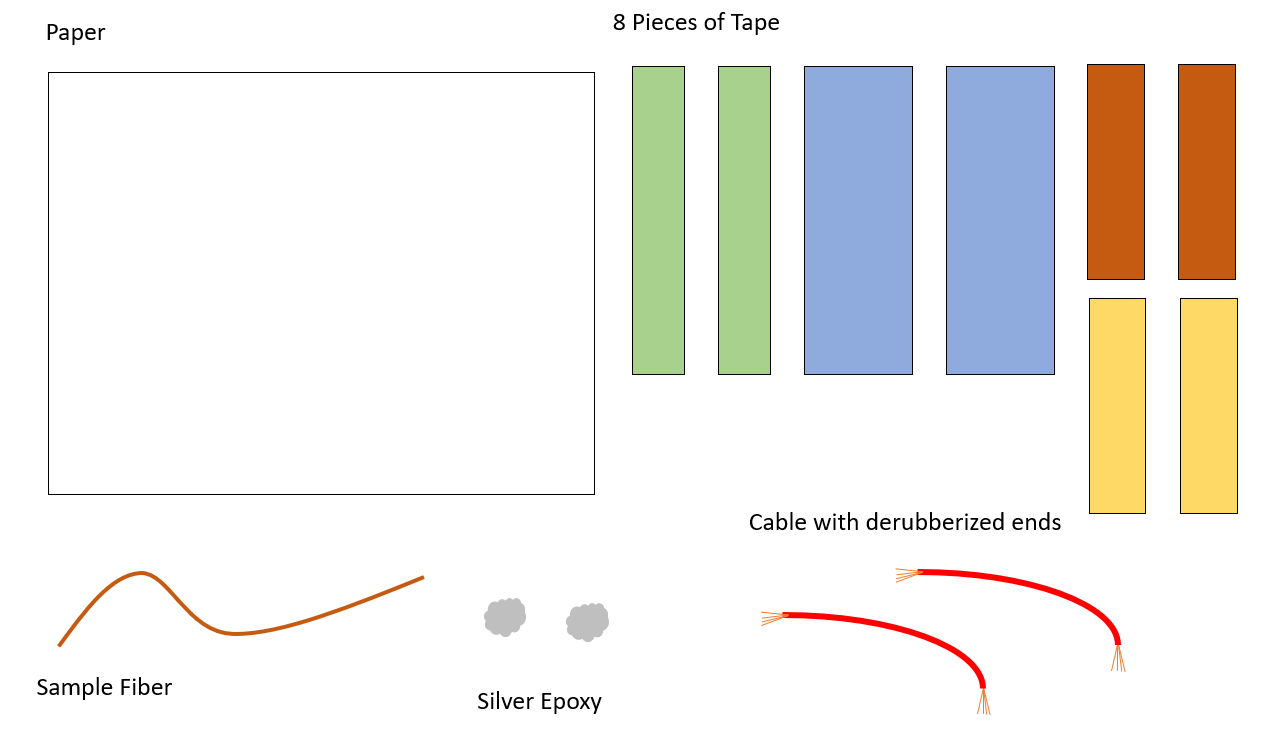
\includegraphics[width=.4\textwidth]{Meas_Prep_1.PNG}
    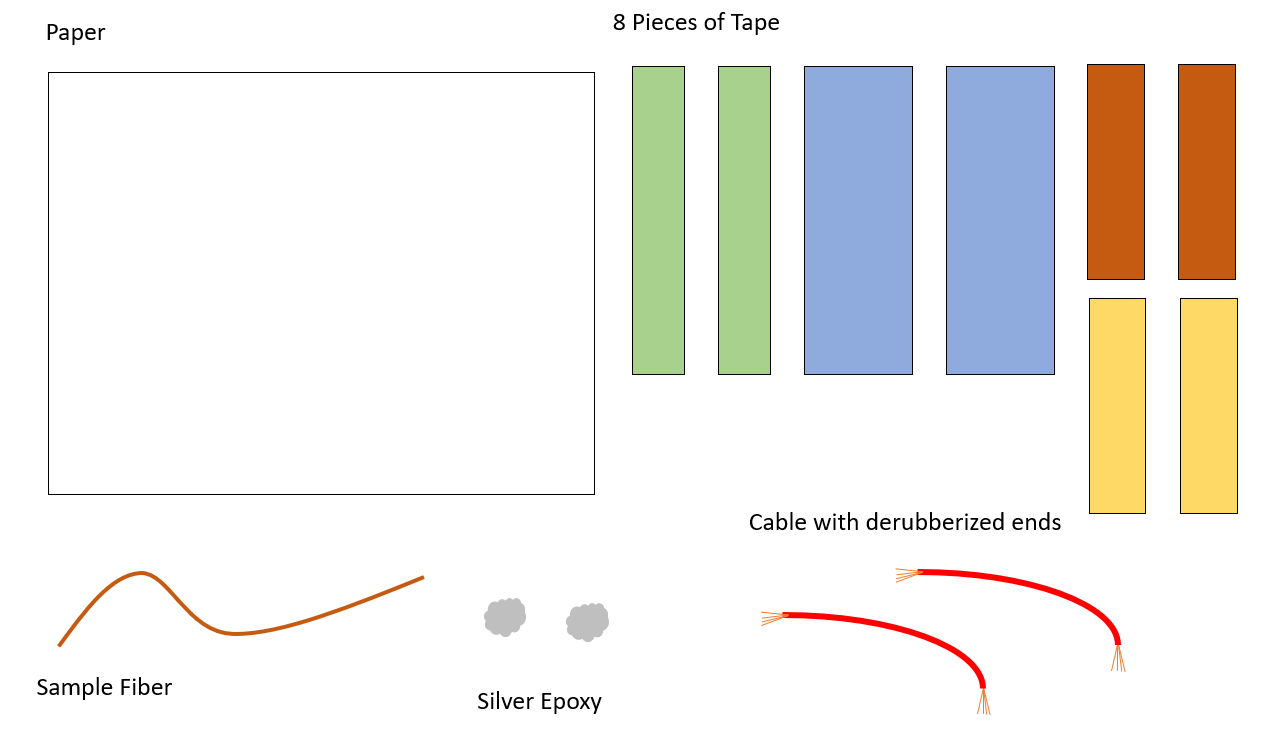
\includegraphics[width=.4\textwidth]{Meas_Prep_1.PNG}
    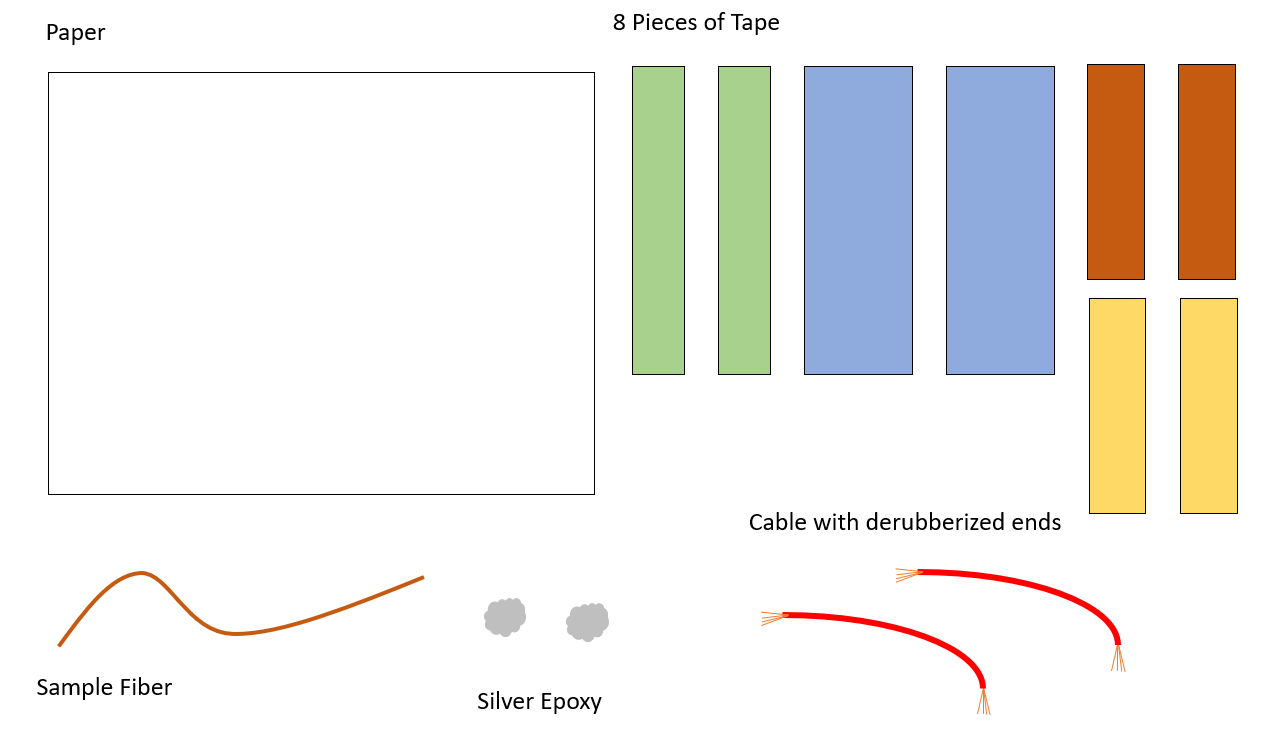
\includegraphics[width=.4\textwidth]{Meas_Prep_1.PNG}
    \caption{Caption}
    \label{fig:my_label}
\end{figure}




\section{\\Cats \& Dogs}
% the \\ insures the section title is centered below the phrase: Appendix B

Text of Appendix B is Here

\end{document}

